\documentclass{article}
\usepackage{fullpage}
%
\usepackage{makeidx}  % allows for indexgeneration
%

\usepackage[draft]{fixme}
\usepackage{color}
\newcommand{\mn}[1]{{\color{red}{#1}}}

\newcommand{\figheight}[1]{55mm}
\newcommand{\figwidth}[1]{0.45\linewidth}
\newcommand{\figfullwidth}[1]{0.9\linewidth}

\usepackage{graphicx}
\graphicspath{{pics/}{figs/}}

\usepackage{amsmath}

\begin{document}
\title{Automatic landmark detection on pediatric airways}
\author{Chun-Wei Liu}
\maketitle              % typeset the title of the contribution

\begin{abstract}
The analysis of pediatric airways using computed tomography (CT) images has provided rich diagnostic cues for doctors. The analysis typically needs proper annotations of visually salient landmarks on CT images. Currently, the annotation works are relied on experts' manual eyeballing. In this work, I introduced the landmark prediction pipeline to pediatric airways from the computer vision community for reducing the annotation cost. To the best of my knowledge, this is the first attempt of landmark detection on pediatric airways. Qualitative and quantitative experiments are performed in the real world dataset. In some cases, the system successfully detected the target landmark within a validated threshold.
\end{abstract}

\section{Introduction}
\label{sec:intro}

The analysis of pediatric airway geometry using 3D computed tomography (CT) images has provided rich cues for doctors to diagnose respiratory issues for patients.
Recently, 4D CT imaging, i.e. a set of 3D CT images, has provided a better characterization of pediatric airways throughout the breathing cycle, for example to assess tracheomalacia, which is a disease causing a temporary collapse of the partial airway.
The advance of medical imaging techniques boost the amount of medical image data in recent year, which brings new challenges on medical image analysis.

One challenge is the landmark annotation.
To analyze different subjects with huge variety using CT images, some pivots with distinguish appearance or shape, i.e. landmarks, have to be placed for registration.
For example, Hong et al. proposed a simplified airway model to represent an airway as a one dimensional cross-sectional area curve.
They used pivots, such as true vocal core (TVC) and trachea carina (TC), to identify the structure in the one dimensional curve.
Therefore, by using the landmark-based registration, they resolved the difficulty of image registration and surface registration between different subjects~\cite{hong2014statistical}.

Currently, for most analysis, landmarks were manually placed by exports.
With the increase amount of medical image data, the annotation costs raises quickly.
To reduce the manual annotation costs in the medical imaging analysis, we need an automatic landmark detection system for these medical image data.

In the medical imaging community, the issues of landmark detection have been addressed in MR brain image using regression forest~\cite{han2014robust} and in lung CT images for surface-based registration~\cite{ehrhardt2010automatic}.
The regression forest learned a non-linear mapping function of the displacement between an image voxel to a hidden landmark voxel.
This method relied on a set of linearly aligned training images.
In my case, the alignment between pediatric airways itself is a difficult problem.
So obtaining a set of aligned training images is infeasible.
On the other hand, the landmark detection algorithm applied on lung images is just for some distinguish local points.
The visually salient landmarks such as TVC or TC in airways cannot be found using such method.

Borrowing the concept of object detector from the computer vision community, I proposed an automatic landmark prediction framework for pediatric airways data, which does not need a set of pre-aligned images.
The framework including two stages: the {\it training} stage and the {\it prediction} stage. Figure~\ref{fig:pipeline} illustrates the framework of the landmark prediction system.

\begin{figure}[tb]
  \begin{center}
    \begin{tabular}{c}
    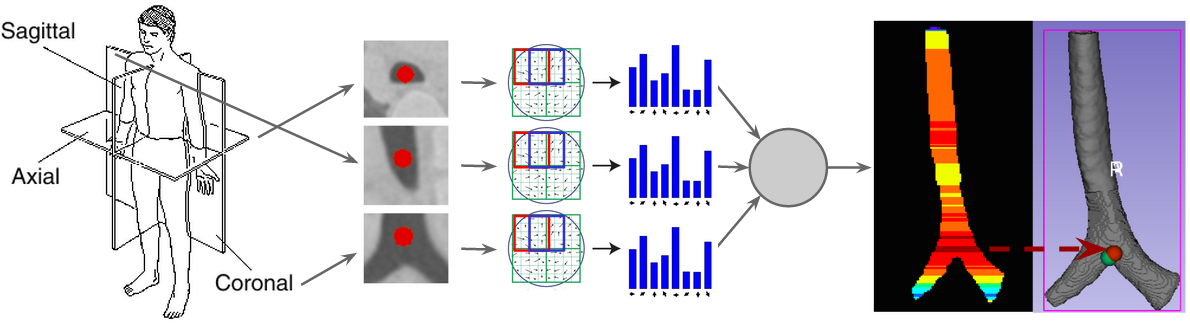
\includegraphics[width=\figfullwidth] {fig/pipeline.png}
    \end{tabular}
    \caption{ \label{fig:pipeline} Visualization of the training and the prediction stages of the proposed landmark detection system. In the training stage, the system extracted the histogram of oriented gradients (HOG) features at the annotation from the axial, sagittal, and cornonal planes of training samples as positive examples, and extracted the HOG features from arbitrary places without overlapping with the bounding box of the positive features as negative features. Then the system trained a binary classifier using linear Support Vector Machine (SVM). In the prediction stage, the framework applied the trained SVM on the candidate locations in the airway using the segmentation. The highest response of the SVM is predicted as the landmark. This figure illustrates the prediction result of Fleck 004. The displacement from the prediction (the red dot) to ground truth (the green dot) is 1.97 (mm).
    }
  \end{center}
\end{figure}

\section{Method}
\label{sec:method}

The landmark predication problem can be formulated as a binary classification problem with label $y$ and features $x$.
We will use $y \in \{-1,1\}$ to denote the class labels. 
I use linear Support Vector Machine (SVM), which has parameters $w$ and $b$, and can be expressed as
\[
h_{w,b}(x) = g(w^Tx + b).
\]
Here, $g(z)=1$ if $z \geq 0$, and $g(z)=-1$ otherwise.
Given a training set $S=\{(x^i,y^i); i=1,\ldots,m\}$, the function margin of $(w,b)$ with respect to S is denoted as $\gamma^i$
\[\gamma^i = y^i(w^Tx+b).\]
A linear SVM solve the following optimization to get the hyperplane with a maximal margin among the data set $S$
\begin{equation*}
\begin{aligned}
& \underset{\gamma,w,b}{\text{minimize}}
& & \frac{1}{2}||w||^2 \\
& \text{subject to}
& & y^i(w^Tx^t + b) \geq 1, \; i = 1, \ldots, m.
\end{aligned}
\end{equation*}


\subsection{Concatenated histogram of gradient}
I proposed the concatenated histogram of oriented gradient (CHOG) as the feature of the framework.
The intuition behind the proposed feature is representing the appearance of the landmark in which experts saw in their manual annotation processing.
An annotation were placed by an expert's eyeballing from three different perspectives: the axial, the sagittal, and the cornonal planes.
A two dimensional feature descriptor is need for the representation of each perspective.

Histogram of oriented gradient (HOG) is widely used in computer vision.
The technique counts occurrences of gradient orientation in localized portions of an image.
The descriptor is suitable for describing object with distinguish shape.
For example, the TC is located at an obvious Y-shape junction.
So the design is expected to work.

\subsection{Training and prediction stages}
To train a binary classifier, I drew positive examples from a set of training subjects with ground truth annotations.
A positive example is a CHOG feature extracted by a local patch containing the annotation.
The length of the local patch is computed by two times of the bounding box of the cross-section of the airway in the axial plane. 
This makes sure the local patch was not just covering airway but the appearance near by the airway.
A negative example is a CHOG feature extracted by an arbitrary location which has no interaction with the positive example.
For each subject in the data set, I gathered a positive example and ten times of negative examples for training.
A linear SVM then was trained by these training examples.

In the prediction stage, I applied the trained SVM to the CT image.
Typically the image size was $512\times512\times640$.
To reducing the hypotheses in a such huge space, I only drew hypotheses of the landmark inside the airway, which needs applying an image segmentation for the airway before the detection.
I drew each hypothesis along with the normal from axial plane since the airway was particular to the axial plane.
Yet this could be viewed as a heuristic.

\section{Results}
I trained a detector on 95 annotated CT images for a particular landmark TC, and tried to predict TC on 7 dynamic CT images (total 94 CT images).

\begin{figure}[tb]
  \begin{center}
    \begin{tabular}{c}
    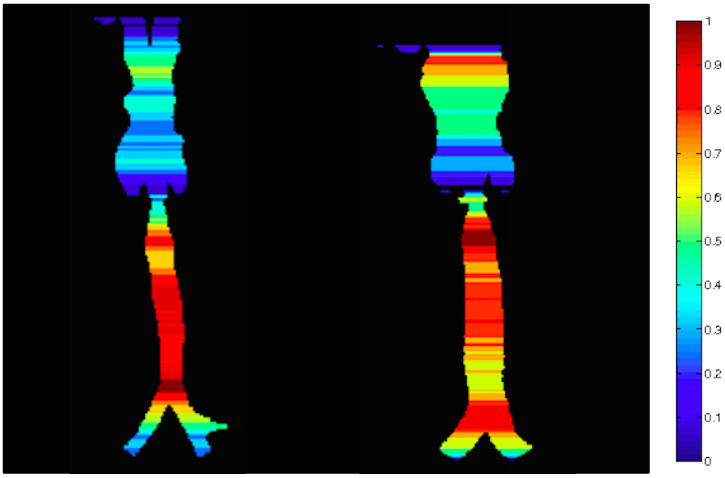
\includegraphics[height=\figheight] {fig/qualitative.png}
    \end{tabular}
    \caption{ \label{fig:qualitative} Qualitative result of the landmark prediction system. Left: A successful case correctly predicted the landmark TC on the airway. Right: A failed case predicted the landmark TC wrong on the airway. The color bar indicates the score of the landmark TC, higher representing higher probability of the prediction. TC should be in the Y-junction of the airway.
    }
  \end{center}
\end{figure}

Figure~\ref{fig:qualitative} shows qualitative results on two training images.
One is a successful case and the other is a failed case.
In the successful case, the prediction error of the TC is within a small range.
In the failed case, the prediction is far away from the ground truth in the bottom of the Y-junction.
However, we can observe even in such a failed case, the prediction score of the Y-junction was still higher than many other hypothesis.

\begin{table}
  \centering
  \begin{tabular}{|lcc|c|c|c|c|}
  \hline
  \multicolumn{3}{|c|}{Subjects} & \multicolumn{2}{|c|}{Landmark Dynamics} & \multicolumn{2}{|c|}{Landmark Prediction} \\
  \hline
  Id  & Age (m) & Weight (kg) & mean & std. & mean & std. \\
  \hline
  Fleck 004 & 134.4   & 39.9  & 4.75 & 2.53 & 3.92 & 4.46 \\
  Fleck 007 & 114     & 25.2  & 4.21 & 6.16 & 7.58 & 5.92 \\
  Fleck 008 & 129.6   & 48.6  & 4.48 & 2.02 & 23.76 & 27.83 \\
  Fleck 009 & 130.8   & 37    & 1.85 & 1.35 & 30.32 & 3.16 \\
  Fleck 010 & 135.6   & 43.9  & 1.93 & 1.03 & 21.21 & 15.34 \\
  Fleck 012 &  42     & 14.5  & 1.48 & 1.03 & 1.47 & 0.69 \\
  Fleck 013 &  21.6   & 16.8  & 0.89 & 0.85 & 23.31 & 9.06 \\
  \hline
  \end{tabular}
  \caption{Qualitative measurement of the landmark detection. The prediction errors should be lower than the landmark dynamics. Currently, the detector only met this standard on the subjects Fleck 004 and Fleck 012.
   }
  \label{tab:Fleck_landmarks}
\end{table}

Table~\ref{tab:Fleck_landmarks} shows quantitative results on the testing images.
Each row is a subject with a dynamic CT scan.
The subject was breathing during the scans so the data reflected the dynamic of the subject.
The landmark dynamics can be computed as the displacement of the landmark between the first frame and the rest of frames.
The landmark prediction errors are listed in the less two columns.
The mean and standard divination (std.) of the landmark dynamics and the prediction errors are listed in the table.
Fairly speaking, a subject with the landmark prediction errors smaller than the landmark dynamics could be considered a successful case.
In our result, only the Fleck 004 and Fleck 012 met this standard.

Some possible explanations for these results:
\begin{enumerate}
\item {\bf Curse of the dimensionality.}
The number of CHOG feature in my experiment is 273.
The 95 positive examples drown from the training set might not enough.
This is a high dimension low sample size statistical analysis.
The classifier might be improved by Distance Weighted Discrimination~\cite{marron2007distance}.
\item {\bf Invalid heuristics.}
The heuristic of drawing hypotheses in the prediction might be invalid.
The airway might not always be perpendicular to the axial plane.
In such situation, an affine transformation might need to apply on the image before extracting the feature.
\item {\bf Geometry prior.}
From Figure~\ref{fig:qualitative}, we see the score of the Y-junction in the failed case is not low.
We should applied geometry prior on the current prediction to increase the probability in the bottom of the airway for the TC.
This would be feasible for some particular landmarks.

\end{enumerate}

\section{Conclusion}
In this work, I introduced the object detection pipeline from the computer vision community to pediatric airways.
I extended the feature from 2D to 3D and implemented a landmark detection framework including training and prediction stages on real world data.
Experiments showed some exciting results but also pointed out the system has a space of improvement.
In the future, I plan to improve the framework by revisiting the three potential issues of curse of the dimensionality, the prediction heuristics, and the geometry prior of the pediatric airways.

\bibliographystyle{splncs}
\bibliography{prp}

\end{document}
